\section{Experimental results of the optical ultrasonic detection system}
\label{sec:OUSDresults}
Based on the calculations and considerations a system for optical ultrasonic detection was built. In the following measurements the results, that characterize the detector, are represented.

\subsection{Finesse}

An important value for the characterization of a FPI is its finesse $\mathcal{F}$. That is defined by

\begin{equation}
\mathcal{F} = \frac{\Delta f}{\mathrm{d} f}
\label{eq:finesse}
\end{equation}
\\
there $\Delta f$ is the distance between two modes and $\mathrm{d} f$ FWHM \cite{eichler:laser}. A higher value here means that more beams inside the resonator sum up with each other, before the light leaves the system.\\
In figure \ref{fig:finesseSimMax} a simulation were done with the values determined above. Therefore the calculated finesse is 14.05. This is the maximum possible finesse achievable with the built system and for a distance of 23~$mm$ between the mirrors.  

\begin{figure}[H]			
	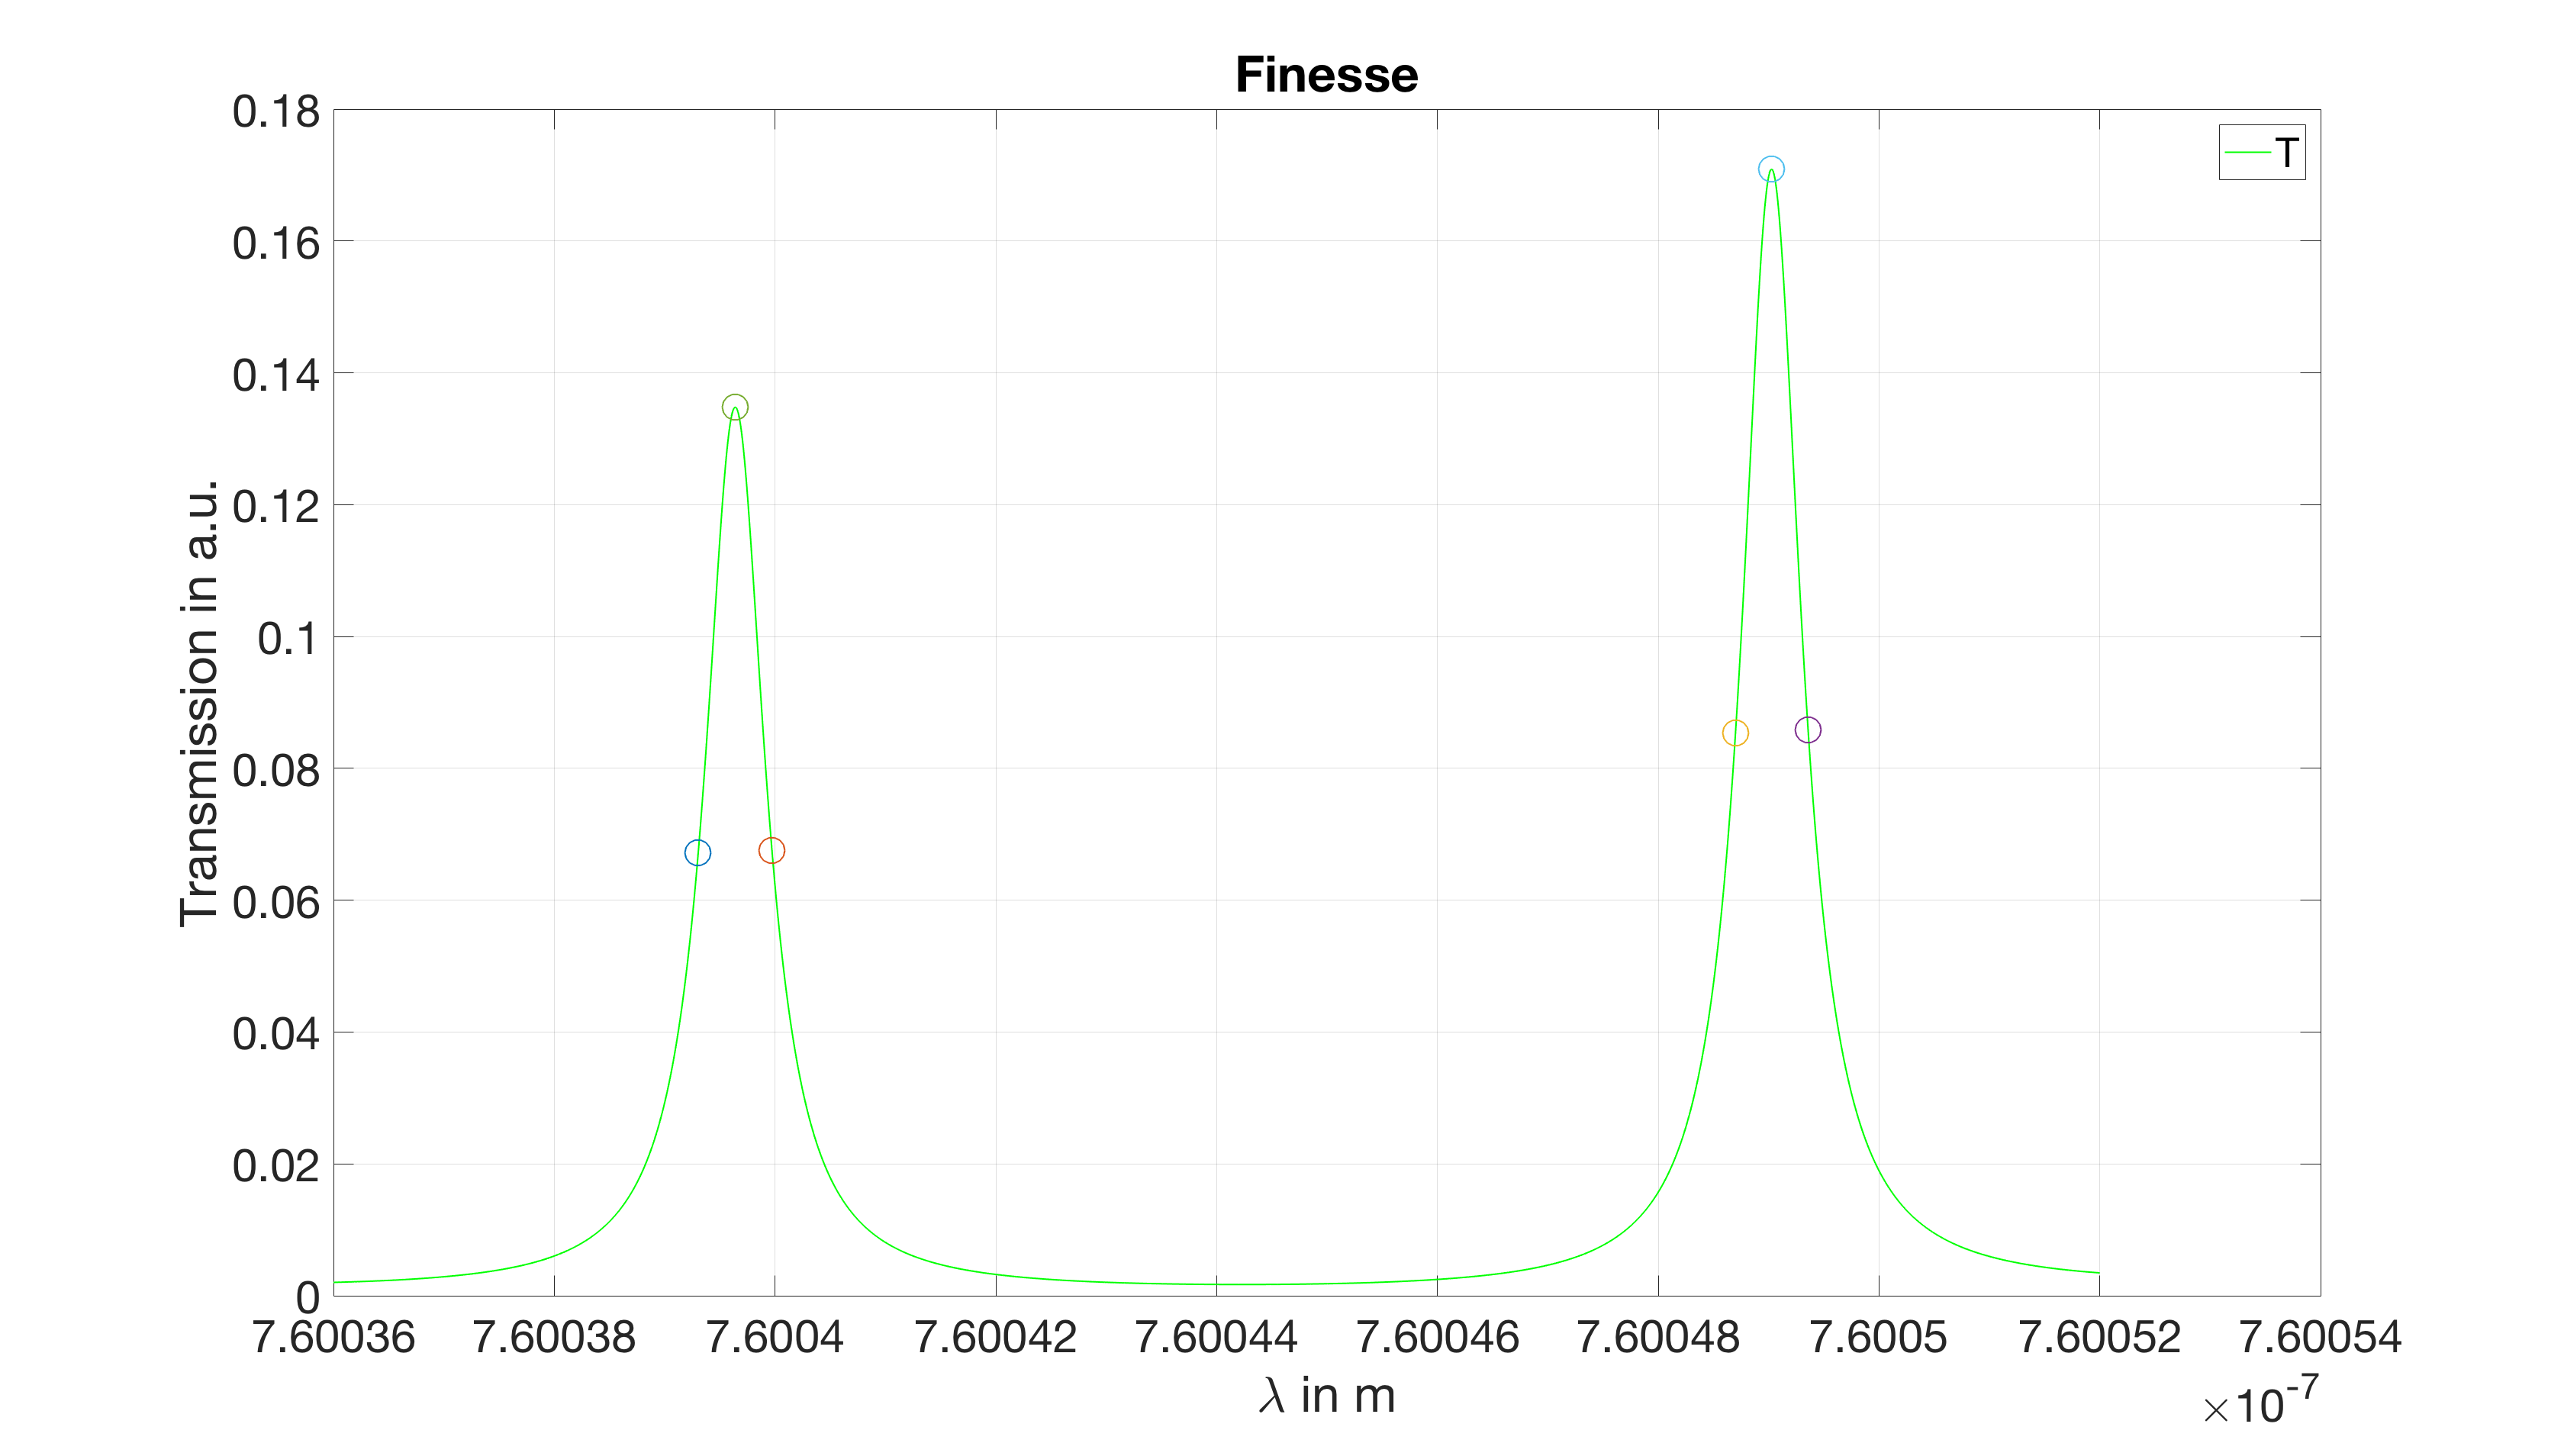
\includegraphics[width = \textwidth, height=0.35\textheight]{06_ex-results_of_OUSD/images/calcFinesse.png}
	\caption{Simulated Transmission pattern for a 30~$nm$ gold layer. The points taken for the measurement of the maximum possible resonator finesse are circled.}
	\label{fig:finesseSimMax}
\end{figure}

It became apparent that the chosen value of 23~$mm$ were too close to the concentric case and therefore to instable. Beside that it is difficult to match the focal points of the mirrors with the flanges screws at that value. In order to determine a more suitable distance a test setup were built.\\
Therefore, the mirrors were mounted onto cage-system bars to change the distance between them. In order to vary the resonance condition one mirror were attached to a piezo-element, that were connected to a waveform generator and the other one were fixed. It is important to note that a laser with 532~$nm$ were used. The reflectivity of the gold coated mirrors is significantly lower compared to 670~$nm$ (see figure \ref{fig:CoatingMat}). However, the influence at this wavelength, to the distance determination, is minimal but the actual finesse value for the OUSD system is higher. \\

\begin{figure}[H]
	a)
	\begin{minipage}{\textwidth}
		\begin{center}		
		\includegraphics[width = 0.85\textwidth, height=0.3\textheight]{06_ex-results_of_OUSD/images/finesse532.png}
		\end{center}
	\end{minipage}
	b)
	\begin{minipage}{\textwidth}
		\vspace*{0.5cm}
		\begin{center}		
		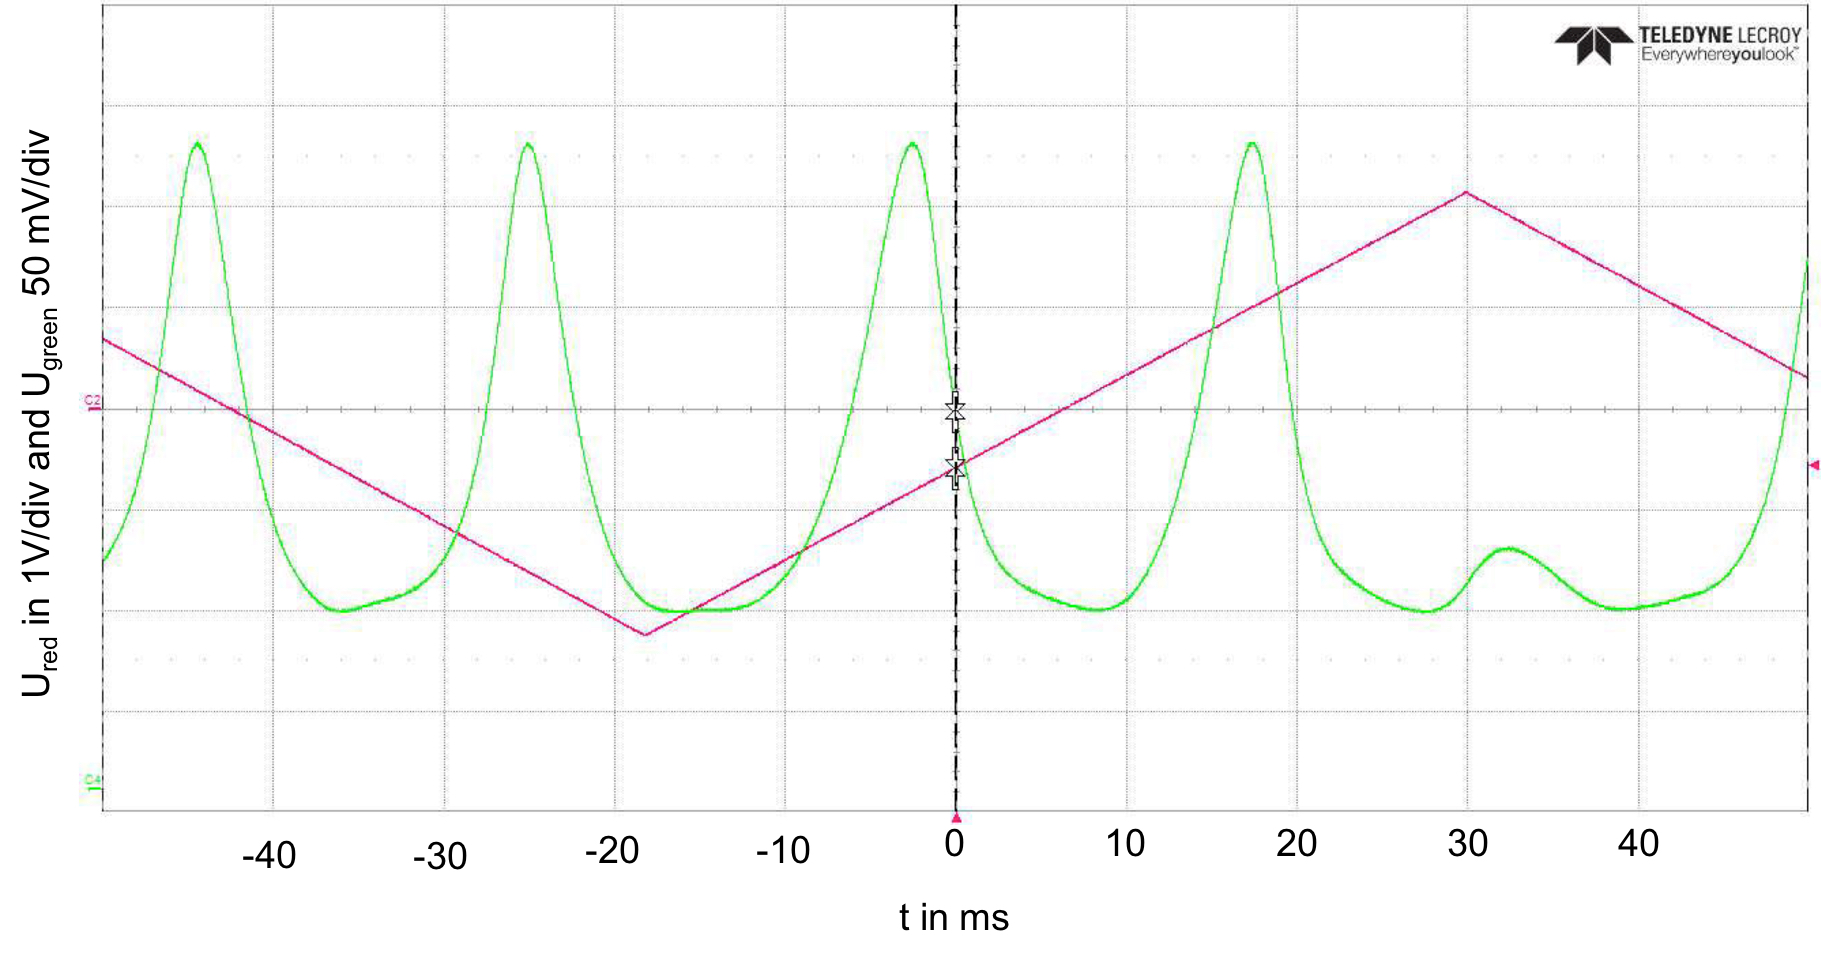
\includegraphics[width = 0.85\textwidth, height=0.3\textheight]{06_ex-results_of_OUSD/images/measFinesse.jpg}
	\end{center}
	\end{minipage}
\caption{In a) a calculated transmission pattern for a mirror distance of 15~$mm$ is displayed. The finesse value is 4.54. Furthermore, b) shows a measured transmission pattern, the finesse is about 4 to 5.}
\label{fig:finesse}
\end{figure}

In figure \ref{fig:finesse} a) a simulation and in b) a measurement of the transmission pattern is shown. The distance between the mirrors were 15~$mm$. Furthermore, the calculated finesse value of figure \ref{fig:finesse} a) agrees with the measured one.\\
As shown in b) a triangular function, for the function generator, were used for the measurements. Due to the shape of the applied voltage the mirror movement follows and the interference condition changes.\\
It turned out that 15~$mm$ also works well in the OUSD system. At that value, the estimated cutoff frequency decreases to about 10~$MHz$, but the positioning of the partially transmitting mirrors and support optics, were easier.\\

\begin{figure}[H]
	a)
	\begin{minipage}[c]{\textwidth}	
		\begin{center}	
		\includegraphics[width = 0.85\textwidth, height=0.3\textheight]{06_ex-results_of_OUSD/images/finesse760.png}
	\end{center}
	\end{minipage}
	b)
	\begin{minipage}[c]{\textwidth}	
		\vspace*{0.5cm}
		\begin{center}
		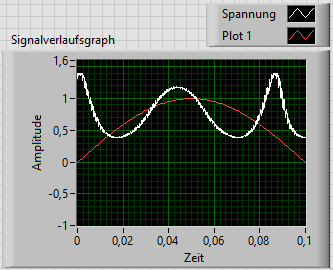
\includegraphics[width = 0.5\textwidth, height=0.25\textheight]{06_ex-results_of_OUSD/images/res_air_piezo@1V.png}
	\end{center}
	\end{minipage}
	\caption{In a) the theoretical possible finesse value for $\lambda$ = 760~$nm$, a mirror distance of 15~$mm$ and water as material between the mirrors. Furthermore, in b) a measured transmission pattern of the OUSD setup is shown. The piezo-element, that moves the grating of the wavelength turnable laser, is sensitive to edged signal sequences, a sinusoidal waveform were chosen.}
	\label{fig:finesseMeas}
\end{figure}

Figure \ref{fig:finesseMeas} b) shows a measured signal of the OUSD with a mirror distance of 15~$mm$ and water as medium between the mirrors. Moreover, the tunable laser system with 760~$nm$ wavelength were used. The finesse is about 6 to 7.\\
To sum up the finesse values, determined in figure \ref{fig:finesse}, for the calculated and measured finesse value agree. Therefore the system were adjusted close to the theoretical maximum finesse value. However, the calculated value of 15.85 in figure \ref{fig:finesseMeas} a), for the actual OUSD setup, were not reached by the measured value in figure \ref{fig:finesseMeas} b). This is referred to the imprecise mirror mounting system, that uses four M2 screws on each flange to fix and position the mirrors.  

\subsection{Transfer function}
\label{sec:OUSDtf}

The transfer function describes the reaction of the OUSD system to an pressure wave with a certain frequency bandwidth. In order to analyze the behavior, four ultrasonic transducers with a defined frequency of 1~$MHz$, 2~$MHz$, 4~$MHz$ and 25~$MHz$ are acoustically coupled onto the system and the response was recorded.\\
The recorded signals were normalized to the maximum pressure amplitudes estimated with the needle hydrophone and the Mach-Zehnder interferometer. Therefore, table \ref{tab:pressureVal} shows the measured data, determined with the methods introduced in chapter \ref{sec:pMeasureMeth}.

\begin{table}[H]
	\centering
	\caption{Measured maximum pressure amplitude for a 1~$MHz$, 2~$MHz$, 4~$MHz$ and 25~$MHz$ ultrasonic transducer. The 25~$MHz$ value for the needle hydrophone is not available, because the cutoff frequency of this device is 10~$MHz$.}
	\begin{tabular}{| m{3cm} | c | c | c | c |}
		\hline
		\centering &1~$MHz$&2~$MHz$&4~$MHz$&25~$MHz$ \\ \hline
		\centering Needle hydrophone&4.37~$kPa$&8.77~$kPa$&7.87~$kPa$&-\\ \hline
		\centering Mach-Zehnder \newline interferometer&4.23~$kPa$&5.79~$kPa$&8.56~$kPa$&8.91~$kPa$\\ \hline
	\end{tabular}

	\label{tab:pressureVal}
\end{table}
The system response to the ultrasonic transducers excitation is recorded and displayed in figure \ref{fig:transF}. The length between the mirrors is 15~$mm$.

\begin{figure}[H]			
	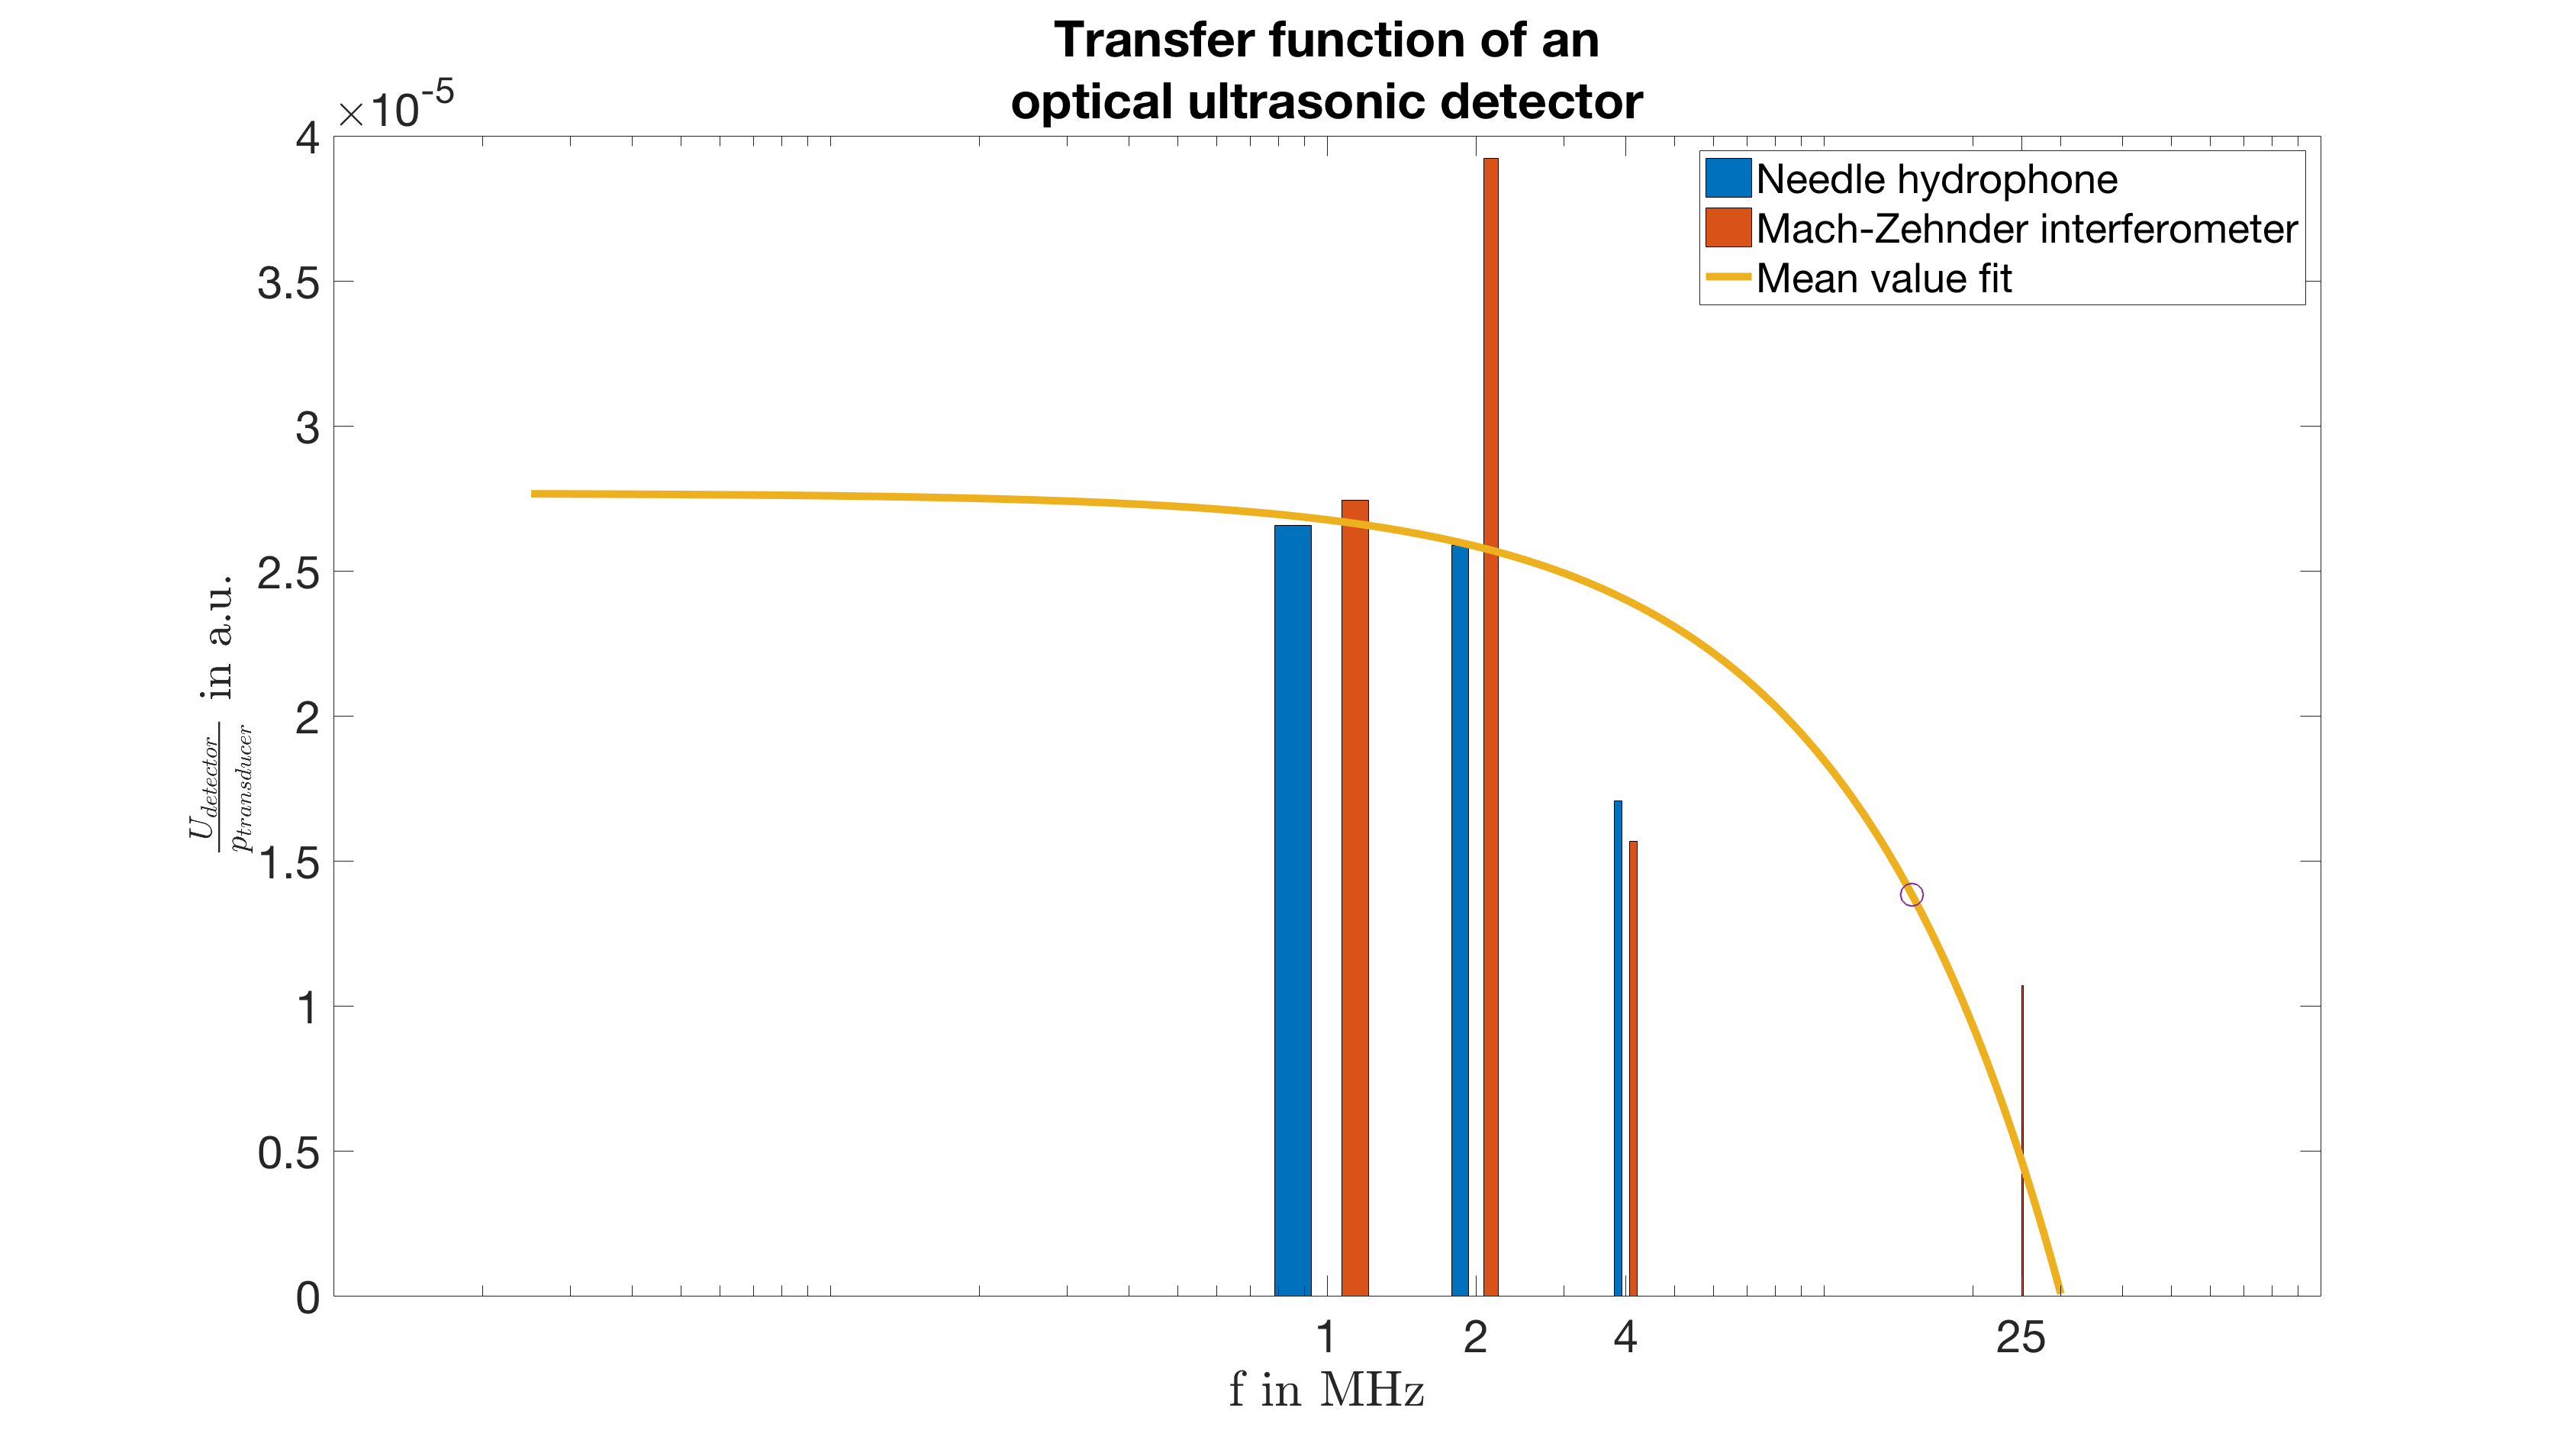
\includegraphics[width = \textwidth, height=0.4\textheight]{06_ex-results_of_OUSD/images/transF.png}
	\caption{Measured transfer function of the OUSD on a half logarithmic scale. The signal amplitudes are normalized to the needle hydrophone data (blue bars) and to the Mach-Zehnder-interferometer data (red bars). The yellow line marks a fit through the mean values and the -3~$dB$ value is marked by a red circle.}
	\label{fig:transF}
\end{figure}

The yellow line in figure \ref{fig:transF} is the fit function ($F_{fit}(f) = -9.2\cdot10^{-7}~\frac{1}{MHz} \cdot f + 2.8\cdot10^{-5}$) through the mean values. These are taken separately for each frequency, only the value for 25~$MHz$ is set to the value of the Mach-Zehnder interferometer. The 3~$dB$ cutoff frequency value is 15.04~$MHz$ which is higher than the estimated 10~$MHz$.\\
For a precise estimation of the cutoff frequency value more datapoints are necessary. But the estimated value lays in the area of the fitted data. 
